\documentclass[main.tex]{subfiles}

\begin{document}

\section*{Goal}
Today we will study an elastic collision and measure the change in momentum during the collision as well as the impulse. Then we will investigate Newton's Third Law by looking at the forces acting on two carts as they interact during a collision.

\section*{Equipment}
\begin{itemize}
\item
850 Universal Interface
\item
PASCO Capstone Software
\item
Motion Sensor, two Force Sensors
\item
Dynamics Track, two carts with rubber bumpers
\item
Lab post for mounting Force Sensor
\item
Mass hanger, masses
\item
Triple-beam balance
\item
Mass bar
\end{itemize}•

\section*{Theory}
In a similar way that we developed the Work-Energy Theorem last time, we can develop what is called the Impulse-Momentum Theorem. First though, let's define what we mean by momentum. \emph{Momentum} is the product of mass and velocity,
\begin{equation} \label{eq:momentum}
\mathbf{p}=m\mathbf{v}.
\end{equation}
Under a collision an object will undergo a change in momentum, which requires a force applied on the object. We can relate an applied force at a specific instant of time to the change of momentum through the following,
\begin{equation} \label{eq:SecondLaw}
\mathbf{F}_{net}=m\mathbf{a}=m\frac{d\mathbf{v}}{dt}=\frac{d}{dt}(m\mathbf{v})=\frac{d\mathbf{p}}{dt},
\end{equation}
which as it turns out is how Newton originally stated his second law of motion in \emph{Principia}. As usual in calculus notation, $d\mathbf{p}$ and $dt$ refer to infinitely small changes of $\mathbf{p}$ and $t.$ Using this we can now define the impulse of the force over a finite interval of time $\Delta t$ as,
\begin{equation} \label{eq:Impulse}
\mathbf{J}=\mathbf{F}_{net}\Delta t,
\end{equation}
provided $\mathbf{F}_{net}$ is a constant force. Using what we know from Equation~\eqref{eq:SecondLaw} we can show that,
\[
\mathbf{F}_{net}=\frac{\Delta\mathbf{p}}{\Delta t},
\]
which if we substitute into Equation~\eqref{eq:Impulse}, 
\begin{equation} \label{eq:AlgIMT}
\mathbf{J}=\mathbf{F}_{net}\Delta t=\Delta\mathbf{p}=m\mathbf{v}_f-m\mathbf{v}_i,
\end{equation}
a specific case of the Impulse-Momentum Theorem. For a generalized Impulse-Momentum Theorem we need to include cases where the net force is not constant. To do this we simply integrate both sides of Equation~\eqref{eq:SecondLaw} with respect to time,
\begin{equation} \label{eq:CalcIMT}
\int_{t_0}^{t}\mathbf{F}_{net}\;dt=\Delta\mathbf{p}.
\end{equation}
n.b., for those without calculus training, for the purposes of this class to take an integral of a function means to find the area between the curve (in this case $F_{net}(t)$ vs $t$) and the horizontal axis of our graph.

For the second part of the experiment we will be studying Newton's Third Law. This is simply stated as,
\begin{equation}
\mathbf{F}_{12}=-\mathbf{F}_{21},
\end{equation}
meaning that the force of object 1 on object 2 is equal in magnitude but opposite in direction to the force of object 2 on object 1.

\section{Setup I: Colliding one cart into a Force Sensor.}
For this activity, the motion sensor will measure the motion of a cart before and after it collides with a bumper that is mounted on the front of a force sensor. The force sensor will measure the force during the collision. Capstone calculates the velocity of the cart before and after the collision, and the integral of force as a function of time during the collision.
\begin{enumerate}
\item
Connect the Motion Sensor and Force Sensor to the 850UI.
\item
Start Capstone.
\item
Under ``Hardware Setup" add the Motion Sensor and Force Sensor to the appropriate ports.
\item
In the toolbar at the bottom of the window next to the timer, change the focus to the Force Sensor by selecting it in the drop-down box. Now, increase the sampling rate to 500 Hz.
\item
Calibrate the Force Sensor as we did on page~\pageref{page:Calibration}, making sure to set the object's weight as a \emph{negative} value.
\item
Carefully measure the mass of the cart and record it in the data table.
\item
Create a calculated result for the momentum of the cart. To do this, click on the ``Calculator" button on the left.
\item
In the first line type ``Momentum = mass*[Velocity (m/s)‎]" and give it units of ``kg*m/s" (Once ``[" is typed we can simply select ``Velocity" and Capstone will link the appropriate data set for the calculation.)
\item
The second line should now read ``mass =." Type in the mass (in kg) of the cart into this line and give it units of ``kg."
\item
Click on ``Calculator" again to hide the window.
\item
Create a graph of Force vs. Time.
\item
Create a new plot area below the Force vs. Time plot by clicking 
\includegraphics{Add_New_Plot}. Choose Momentum as the vertical axis measurement for this plot.
\item
Mount the Force Sensor horizontally as shown below. Make sure that the rubber bumper is on the end of the Force Sensor's hook.

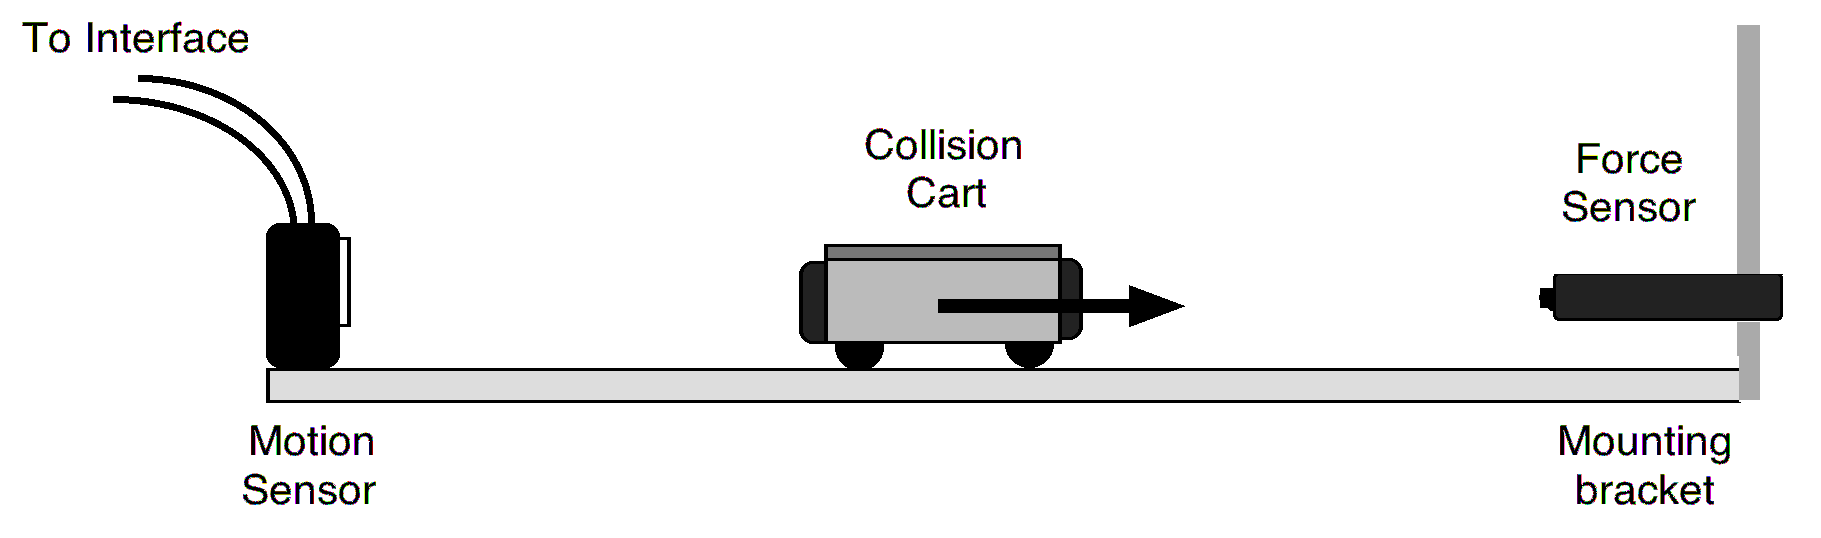
\includegraphics[width=\textwidth]{Imp-Mom_1_Setup}

\item
Raise the end of the track that is opposite to the end with the Force Sensor about 1.5 cm so the cart will have roughly the same initial velocity each trial at the moment it first contact the force sensor.
\item
Place the Motion Sensor at the raised end of the track so that it can measure the motion of the cart.
\item
Brace the Force Sensor end of the track so that the track will not move during the collision.
\end{enumerate}•

\subsection*{Procedure}
\begin{enumerate}
\item
Press the tare button on the side of the Force Sensor to zero the sensor.
\item
Place the cart on the track at least 20 cm from the front of the Motion Sensor.
\item
Click on Record to begin data collection and at the same time release the cart so that it rolls down towards the Force Sensor.
\item
Click on Stop to end the data collection after the cart has rebounded \emph{once} from the collision with the Force Sensor's bumper. n.b., it is best to allow the cart to begin to roll back up the track before ending data collection.
\end{enumerate}•

\subsection*{Analysis}
\begin{enumerate}
\item
Scale the data to fit the graph.
\item
On the Force vs Time graph, click on the Selection Tool, 
\includegraphics{Selection_Tool}. Move and resize the rectangle to only highlight the spike, the region of the graph that corresponds to the collision.
\item
Press the scale to fit button, 
\includegraphics{Rescale}, this will scale the graph to only show the points inside the Selection Tool. Resize the rectangle as needed so that only the spike is included.
\item
Click on the ``Display area under active data" button, 
\includegraphics{Area_Under_Curve}. Record the area in the data table.
\item
On the Momentum vs Time graph, click on the Selection Tool, 
\includegraphics{Selection_Tool} and move the rectangle to highlight the collision which should occur at the same times as it did in the Force vs Time graph. (It isn't critical to have the rectangle perfect for this graph, so long as the collision is included inside the Selection Tool.
\item
Under Statistics 
\includegraphics{Statistics}, check the``Minimum" and ``Maximum" choices and uncheck everything else. Finally click the $\Sigma$ to display the information.
\item
\textbf{Print} a copy of the graph for each group member.
\item
Using the information from the Momentum vs Time graph, calculate the change in momentum.
\item
Calculate the percent discrepancy between the impulse and the change in momentum, holding the impulse as the standard.
\end{enumerate}•

\begin{question}
What is the unit of impulse given in the Force vs Time graph? What is the unit of momentum given in the Momentum vs Time graph? Show that these units are equivalent.
\end{question}
\begin{question}
Why do the maximum and minimum momenta have opposite signs?
\end{question}

\section{Setup II: Collision of Two Carts.}
For this activity, Force sensors are attached to two carts. The carts are placed on a track, and the Force Sensors measure the force of interaction during collisions. Capstone displays Force vs Time for both sensors simultaneously. We will compare the area under the Force vs Time curve for one Force Sensor with the area above the Force vs Time curve for the second Force Sensor.
\begin{enumerate}
\item
Disconnect the Motion Sensor, wrap the cord and put aside.
\item
Connect a second Force Sensor to the 850UI.
\item
Click the New Page button 
\includegraphics{Add_Page} and create a graph.
\item
We will need to display the data from both Force Sensors simultaneously on this graph. Click on the Add New $y$-axis to plot button, 
\includegraphics{Add_New_Y-Axis}.
\item
Select ``Force, Ch A (N)" for one of the axes and ``Force, Ch B (N)" for the other.
\item
As we have already calibrated the Force Sensor in Channel A, we only need to calibrate the sensor in Channel B. Calibrate this sensor as we did before (see page~\pageref{page:Calibration}) however this time make sure that the weight of the mass is recorded as a \emph{positive} value.
\item
Under ``Data Summary" in the toolbar on the left, click on the line labeled ``Force, Ch A (N)" and then click on the Properties button 
\includegraphics{Properties}. In the ``Numerical Format" section, change the Number of Decimal Places to 4. Click ``OK" to close the window. Repeat this step for ``Force, Ch B (N)."
\item
Set up the carts and track as shown below. Make sure that the rubber bumpers are attached to the hooks of the sensors.

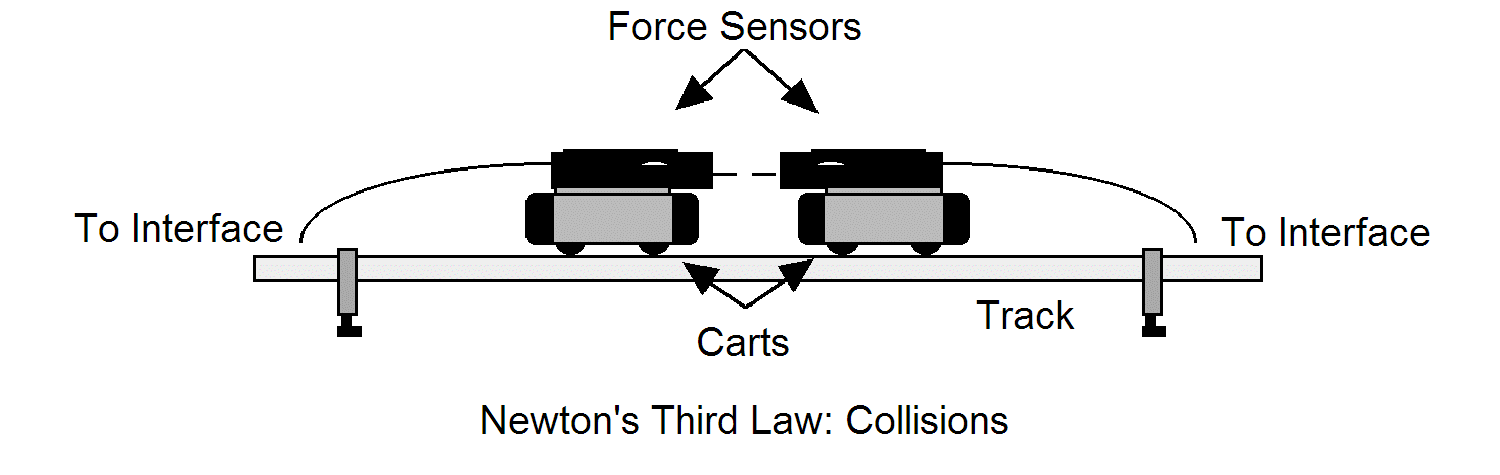
\includegraphics[width=\textwidth]{Imp-Mom_2_Setup}
\end{enumerate}•

\subsection*{Procedure I}
\begin{enumerate}
\item \label{step:Imp-Mom_2a_begin}
For this experiment it is important to zero the sensors by pressing the tare button before we begin data collection each time.
\item
Move the carts to opposite ends of the track.
\item
Click on the Record button. Push the two carts together, allowing them to collide at approximately equal speeds near the center of the track. Click the Stop button to end the data collection.
\item \label{step:Area_of_curves}
On the graph there should be two narrow spikes representing the collision. Use the Selection Tool 
\includegraphics{Selection_Tool} to highlight one of the peaks. As we did in Setup I, use the Scale to Fit 
\includegraphics{Rescale} to help trim the selection so that only the peak is selected. Click the `Display area under active data" button, 
\includegraphics{Area_Under_Curve}. 
\item \label{step:Imp-Mom_2a_end}
Repeat step~\ref{step:Area_of_curves} for the other peak. To switch between data sets, simply click the icon in the legend.
\item
If both peaks look reasonably similar and have minimums of 0 N, then proceed to the analysis. If not, for example there are multiple peaks or one sensor has minimum readings that are not zero., then remove the data and repeat steps~\ref{step:Imp-Mom_2a_begin}--\ref{step:Imp-Mom_2a_end}.
\end{enumerate}•

\subsection*{Analysis}
\begin{enumerate}
\item
Record the areas from both peaks in the data table.
\item
\textbf{Print} the graph for each group member.
\item
Calculate the average impulse readings and enter the result in the data table.
\item
Calculate the \emph{relative} discrepancy. This compares how individual readings differ from the average. Since there are only two readings they have the same relative discrepancy. The equation is defined on page~\pageref{page:Relative_Discrepancy} but we will repeat it here for convenience.
\[
\text{Relative discrepancy } = \frac{|\text{experimental value} - \text{average value}|}{\text{average value}} \times 100\%
\]
\end{enumerate}•

\subsection*{Procedure II}
\begin{enumerate}
\item
Add a mass bar to the cart connected to the Force Sensor in channel A.
\item
Repeat the data collection and analysis from above. Do not print a graph for this run but enter the data and calculations in the data table.
\end{enumerate}•

\subsection*{Procedure III}
\begin{enumerate}
\item
Keep the mass bar on the Channel A cart.
\item
Repeat the data collection and analysis from above. However, this time leave the heavier cart at rest near the middle of the track and only move the lighter cart. Do not print a graph for the run but enter the data and calculations in the data table.
\end{enumerate}•

\subsection*{Procedure IV}
\begin{enumerate}
\item
Keep the mass bar on the Channel A cart.
\item
Repeat the data collection and analysis from above. However, this time leave the lighter cart at rest near the middle of the track and only move the heavier cart. Do not print a graph for the run but enter the data and calculations in the data table.
\end{enumerate}•

\begin{question}
Why is the area under the Force vs Time graph the impulse?
\end{question}
\begin{question}
Which cart experiences more force when both are moving with equal masses?
\end{question}
\begin{question}
Which cart experiences more force when one cart remains at rest? Do the masses of the carts matter? What are the relative discrepancies?
\end{question}

\begin{samepage}
\hrulefill \\ \\
\emph{Chapter~\ref{chap:Imp-Mom}:} \textbf{Impulse \& Momentum}
\begin{enumerate}
\item
\textbf{(1)} Title Page
\item
\textbf{(6)} Purpose of both setups.
\item
\textbf{(12)} Theory --- Should cover both setups.
\item
\textbf{(4)} Data sheets
\item
\textbf{(3)} Graphs
\item
\textbf{(8)} Sample calculations for both setups
\item
\textbf{(10)} Answers to all questions.
\item
\textbf{(6)} Conclusion of both setups.
\end{enumerate}•
\end{samepage}

\newpage
\section{Data Tables}

\subsection*{Setup I}
\begin{doublespace}
\resizebox{0.8\textwidth}{!}{
\begin{tabular}{|l|@{\hskip 2 cm}r|}
\hline
Item & Value\\
\hline
Mass of cart & kg\\
\hline
Impulse & N s\\
\hline
Momentum before collision & kg m/s\\
\hline
Momentum after collision & kg m/s\\
\hline
Percent Uncertainty & \%\\
\hline
\end{tabular}•
}

\newpage
\subsection*{Setup II}
\textbf{Run \#1: Two equal mass carts.}\\
\resizebox{0.8\textwidth}{!}{
\begin{tabular}{|l|@{\hskip 2 cm}r|}
\hline
Impulse of cart \#1 & N s\\
\hline
Impulse of cart \#2 & N s\\
\hline
Average Impulse & N s\\
\hline
Relative Discrepancy & \%\\
\hline
\end{tabular}
}

\noindent
\textbf{Run \#2: Cart \#1 heavier, equal speeds.}\\
\resizebox{0.8\textwidth}{!}{
\begin{tabular}{|l|@{\hskip 2 cm}r|}
\hline
Impulse of cart \#1 & N s\\
\hline
Impulse of cart \#2 & N s\\
\hline
Average Impulse & N s\\
\hline
Relative Discrepancy & \%\\
\hline
\end{tabular}
}

\noindent
\textbf{Run \#3: Cart \#1 heavier and at rest.}\\
\resizebox{0.8\textwidth}{!}{
\begin{tabular}{|l|@{\hskip 2 cm}r|}
\hline
Impulse of cart \#1 & N s\\
\hline
Impulse of cart \#2 & N s\\
\hline
Average Impulse & N s\\
\hline
Relative Discrepancy & \%\\
\hline
\end{tabular}
}

\noindent
\textbf{Run \#4: Cart \#1 heavier, lighter cart at rest.}\\
\resizebox{0.8\textwidth}{!}{
\begin{tabular}{|l|@{\hskip 2 cm}r|}
\hline
Impulse of cart \#1 & N s\\
\hline
Impulse of cart \#2 & N s\\
\hline
Average Impulse & N s\\
\hline
Relative Discrepancy & \%\\
\hline
\end{tabular}
}
\end{doublespace}
\end{document}
